\begin{frame}[fragile]{Multiple Regression Case Study: Motor Trend Cars}
    The \texttt{mtcars} data in \texttt{R} has data on 10 aspects of car design and performance for 32 automobiles:
    \footnotesize{
    \begin{verbatim}
                   mpg cyl disp  hp drat    wt  qsec vs am gear carb
Mazda RX4         21.0   6  160 110 3.90 2.620 16.46  0  1    4    4
Mazda RX4 Wag     21.0   6  160 110 3.90 2.875 17.02  0  1    4    4
Datsun 710        22.8   4  108  93 3.85 2.320 18.61  1  1    4    1
Hornet 4 Drive    21.4   6  258 110 3.08 3.215 19.44  1  0    3    1
Hornet Sportabout 18.7   8  360 175 3.15 3.440 17.02  0  0    3    2
Valiant           18.1   6  225 105 2.76 3.460 20.22  1  0    3    1
    \end{verbatim}}
\end{frame}

\begin{frame}{Example}
    Let's start with examining horsepower and miles per gallon.
    \begin{center}
        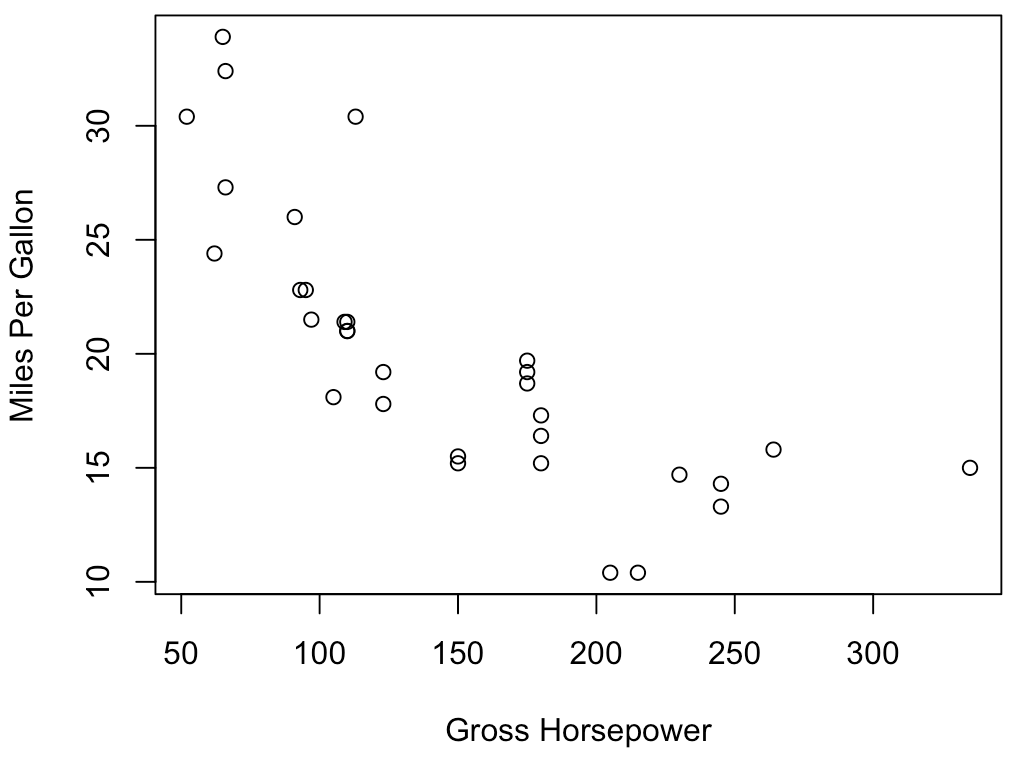
\includegraphics[width=3in]{images/mtcars1.png}
    \end{center}
\end{frame}

\begin{frame}[fragile]{A Simple Linear Model}
    It's hard to tell whether this relationship is linear or not. Let's start with the simple linear model.
    \begin{verbatim}
            Estimate Std. Error t value Pr(>|t|)    
(Intercept) 30.09886    1.63392  18.421  < 2e-16 ***
hp          -0.06823    0.01012  -6.742 1.79e-07 ***

Multiple R-squared:  0.6024,	Adjusted R-squared:  0.5892 
    \end{verbatim}
    Write the regression model. Interpret the coefficients. 
\end{frame}

\begin{frame}[fragile]{A Quadratic Model}
    Now let's try a model with a quadratic term.
    \begin{verbatim}
             Estimate Std. Error t value Pr(>|t|)    
(Intercept)    20.091      0.544  36.931  < 2e-16 ***
hp1           -26.046      3.077  -8.464 2.51e-09 ***
hp2            13.155      3.077   4.275 0.000189 ***

Multiple R-squared:  0.7561,	Adjusted R-squared:  0.7393 
    \end{verbatim}
    Write the regression model.
\end{frame}

\begin{frame}[fragile]{Multiple Linear Regression}
    Now, we know that other variables may be useful... so let's try adding them in. The summary of full model (with \texttt{hp}$^2$ included) is
    \small{\begin{verbatim}
            Estimate Std. Error t value Pr(>|t|)  
(Intercept)   13.982035  18.988291   0.736    0.470
cyl            0.044743   1.041147   0.043    0.966
disp           0.008652   0.018070   0.479    0.637
hp1          -11.877106   8.753289  -1.357    0.190
hp2            4.959203   4.072697   1.218    0.238
drat           0.430521   1.643201   0.262    0.796
wt            -2.967539   1.971111  -1.506    0.148
qsec           0.510263   0.766336   0.666    0.513
vs            -0.190406   2.122169  -0.090    0.929
am             1.748014   2.130010   0.821    0.422
gear           0.927728   1.493229   0.621    0.541
carb          -0.469657   0.848911  -0.553    0.586 
    \end{verbatim}}
    \vspace{-10pt}How many predictors are in this model? What does $\beta_4$ represent?
\end{frame}

\begin{frame}{Example}
    \begin{itemize}
        \item The estimated coefficient for \texttt{hp}$^2$ in the smaller model was 13.155
        \item In the full model, this coefficient is 4.959.
    \end{itemize}
    Why might this difference occur?
\end{frame}

\begin{frame}[fragile]{Model Selection}
    Let's do a backward selection based on p-values.
    \small{\begin{verbatim}
            Estimate Std. Error t value Pr(>|t|)  
(Intercept)   13.982035  18.988291   0.736    0.470
cyl            0.044743   1.041147   0.043    0.966
disp           0.008652   0.018070   0.479    0.637
hp1          -11.877106   8.753289  -1.357    0.190
hp2            4.959203   4.072697   1.218    0.238
drat           0.430521   1.643201   0.262    0.796
wt            -2.967539   1.971111  -1.506    0.148
qsec           0.510263   0.766336   0.666    0.513
vs            -0.190406   2.122169  -0.090    0.929
am             1.748014   2.130010   0.821    0.422
gear           0.927728   1.493229   0.621    0.541
carb          -0.469657   0.848911  -0.553    0.586 
    \end{verbatim}}
    \vspace{-10pt} What variable do we remove first?
\end{frame}

\begin{frame}[fragile]{Model Selection}
    \small{\begin{verbatim}
            Estimate Std. Error t value Pr(>|t|)  
(Intercept)   14.516933  13.994971   1.037    0.311
disp           0.008873   0.016907   0.525    0.605
hp1          -11.796710   8.345344  -1.414    0.172
hp2            4.937641   3.944451   1.252    0.224
drat           0.413058   1.553865   0.266    0.793
wt            -2.979803   1.903425  -1.565    0.132
qsec           0.503152   0.730261   0.689    0.498
vs            -0.216661   1.983443  -0.109    0.914
am             1.728754   2.032237   0.851    0.405
gear           0.904345   1.357122   0.666    0.512
carb          -0.460509   0.802022  -0.574    0.572
    \end{verbatim}}
\end{frame}

\begin{frame}[fragile]{Model Selection}
    \small{\begin{verbatim}
            Estimate Std. Error t value Pr(>|t|)  
(Intercept)   14.922119  13.187937   1.131    0.270
disp           0.009315   0.016044   0.581    0.567
hp1          -11.914838   8.087022  -1.473    0.155
hp2            4.832406   3.738113   1.293    0.210
drat           0.401197   1.514859   0.265    0.794
wt            -2.985060   1.859596  -1.605    0.123
qsec           0.474635   0.666511   0.712    0.484
am             1.774822   1.942840   0.914    0.371
gear           0.874993   1.300039   0.673    0.508
carb          -0.440539   0.763170  -0.577    0.570
    \end{verbatim}}
\end{frame}

\begin{frame}[fragile]{Model Selection}
    \small{\begin{verbatim}
            Estimate Std. Error t value Pr(>|t|)  
(Intercept)   16.176651  12.056492   1.342    0.193
disp           0.009256   0.015714   0.589    0.562
hp1          -12.340452   7.763871  -1.589    0.126
hp2            5.071981   3.552934   1.428    0.167
wt            -3.018258   1.817474  -1.661    0.110
qsec           0.471422   0.652791   0.722    0.477
am             1.848385   1.883611   0.981    0.337
gear           0.953887   1.239606   0.770    0.449
carb          -0.424462   0.745215  -0.570    0.574
    \end{verbatim}}
\end{frame}

\begin{frame}[fragile]{Model Selection}
    \small{\begin{verbatim}
            Estimate Std. Error t value Pr(>|t|)  
(Intercept)   13.41166   10.87958   1.233  0.22961   
disp           0.01510    0.01174   1.286  0.21057   
hp1          -14.31438    6.84901  -2.090  0.04739 * 
hp2            4.62330    3.41540   1.354  0.18846   
wt            -3.76861    1.23435  -3.053  0.00547 **
qsec           0.67281    0.54097   1.244  0.22562   
am             2.00853    1.83611   1.094  0.28486   
gear           0.67669    1.12392   0.602  0.55277
    \end{verbatim}}
\end{frame}

\begin{frame}[fragile]{Model Selection}
    \small{\begin{verbatim}
            Estimate Std. Error t value Pr(>|t|)  
(Intercept)   16.62533    9.35861   1.776  0.08783 . 
disp           0.01200    0.01041   1.152  0.26006   
hp1          -13.19944    6.50931  -2.028  0.05337 . 
hp2            4.79117    3.36032   1.426  0.16629   
wt            -3.66706    1.20708  -3.038  0.00551 **
qsec           0.64249    0.53171   1.208  0.23822   
am             2.52789    1.60007   1.580  0.12671
    \end{verbatim}}
\end{frame}

\begin{frame}[fragile]{Model Selection}
    \small{\begin{verbatim}
            Estimate Std. Error t value Pr(>|t|)  
(Intercept)   20.2315     8.8754   2.280  0.03108 * 
hp1          -11.5546     6.3908  -1.808  0.08219 . 
hp2            4.5925     3.3770   1.360  0.18553   
wt            -2.7832     0.9379  -2.967  0.00637 **
qsec           0.4486     0.5075   0.884  0.38492   
am             1.9866     1.5392   1.291  0.20817 
    \end{verbatim}}
\end{frame}

\begin{frame}[fragile]{Model Selection}
    \small{\begin{verbatim}
            Estimate Std. Error t value Pr(>|t|)  
(Intercept)   27.5420     3.2037   8.597 3.27e-09 ***
hp1          -16.2337     3.5647  -4.554 0.000101 ***
hp2            6.1579     2.8635   2.151 0.040628 *  
wt            -2.4839     0.8711  -2.851 0.008242 ** 
am             1.3289     1.3419   0.990 0.330791 
    \end{verbatim}}
\end{frame}

\begin{frame}[fragile]{Model Selection}
    \small{\begin{verbatim}
            Estimate Std. Error t value Pr(>|t|)  
(Intercept)   29.8389     2.2093  13.506 8.72e-14 ***
hp1          -15.1717     3.3984  -4.464  0.00012 ***
hp2            6.8997     2.7628   2.497  0.01867 *  
wt            -3.0300     0.6741  -4.495  0.00011 ***
    \end{verbatim}}
    Write out the final model.
\end{frame}

\begin{frame}{Diagnostics: Normality}
    Now that we have a final model, we should check our regression diagnostics.
    \begin{center}
        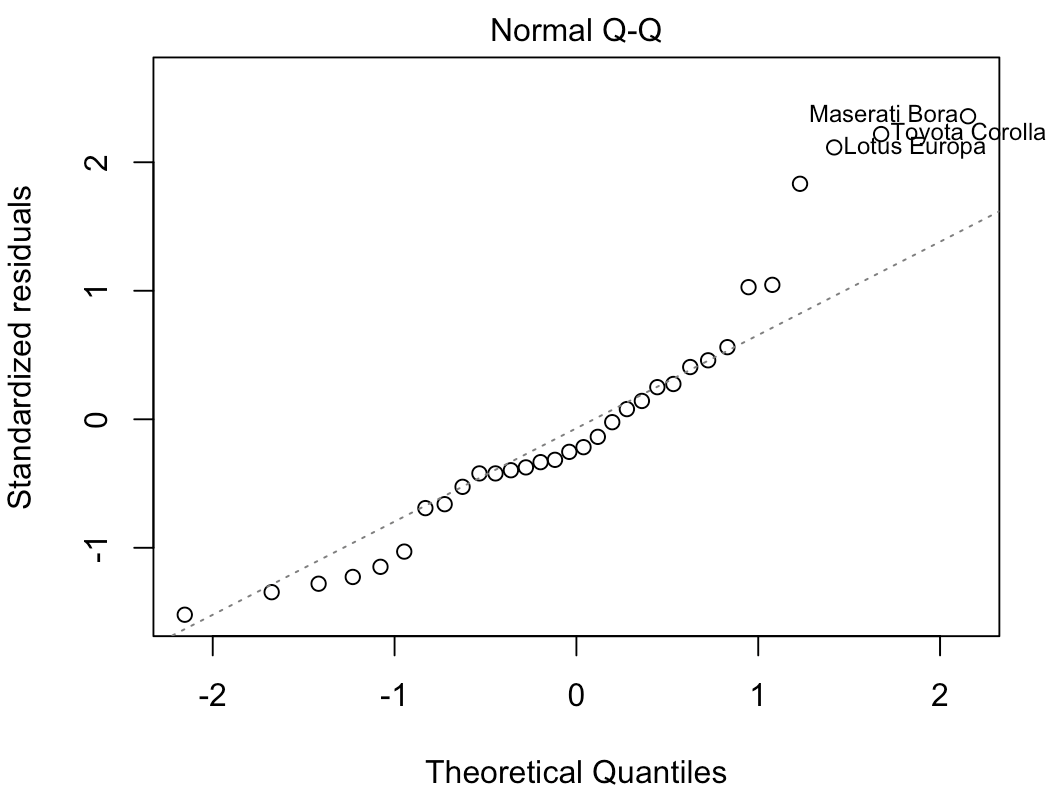
\includegraphics[width=3.5in]{images/mtcarsqq.png}
    \end{center}
\end{frame}

\begin{frame}{Diagnostics: Constant Variance}
    \begin{center}
        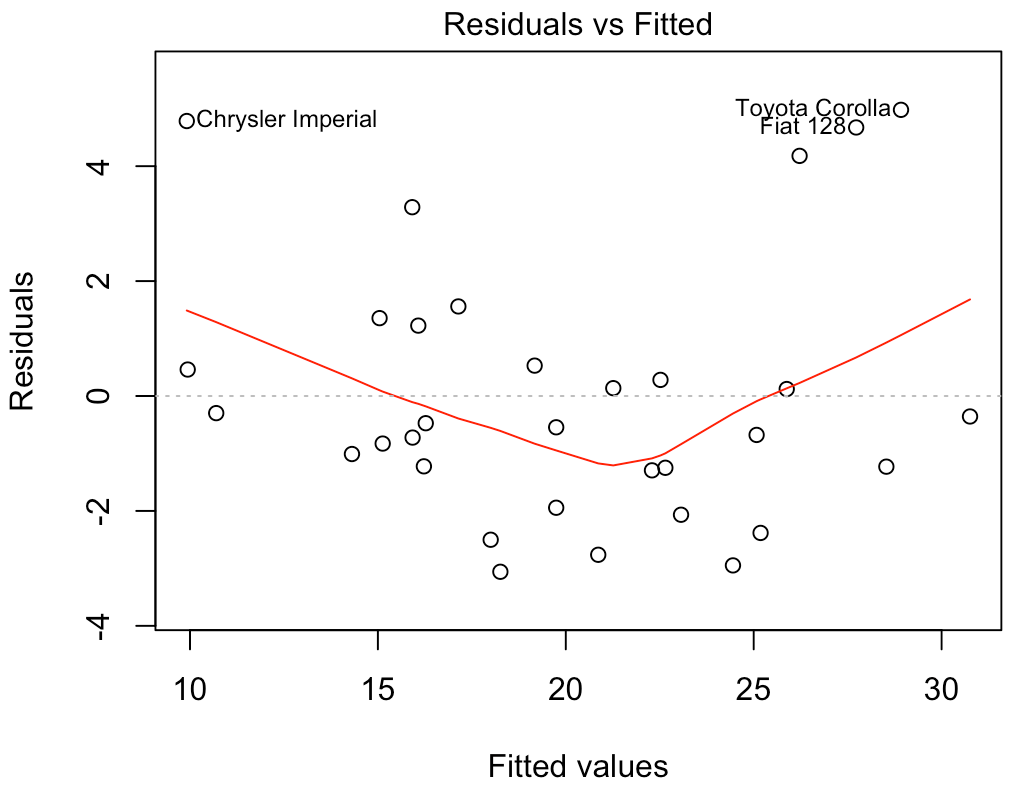
\includegraphics[width=3.5in]{images/mtcarsresidft.png}
    \end{center}
\end{frame}

\begin{frame}{Diagnostics: Residuals vs. Predictors}
    \begin{center}
        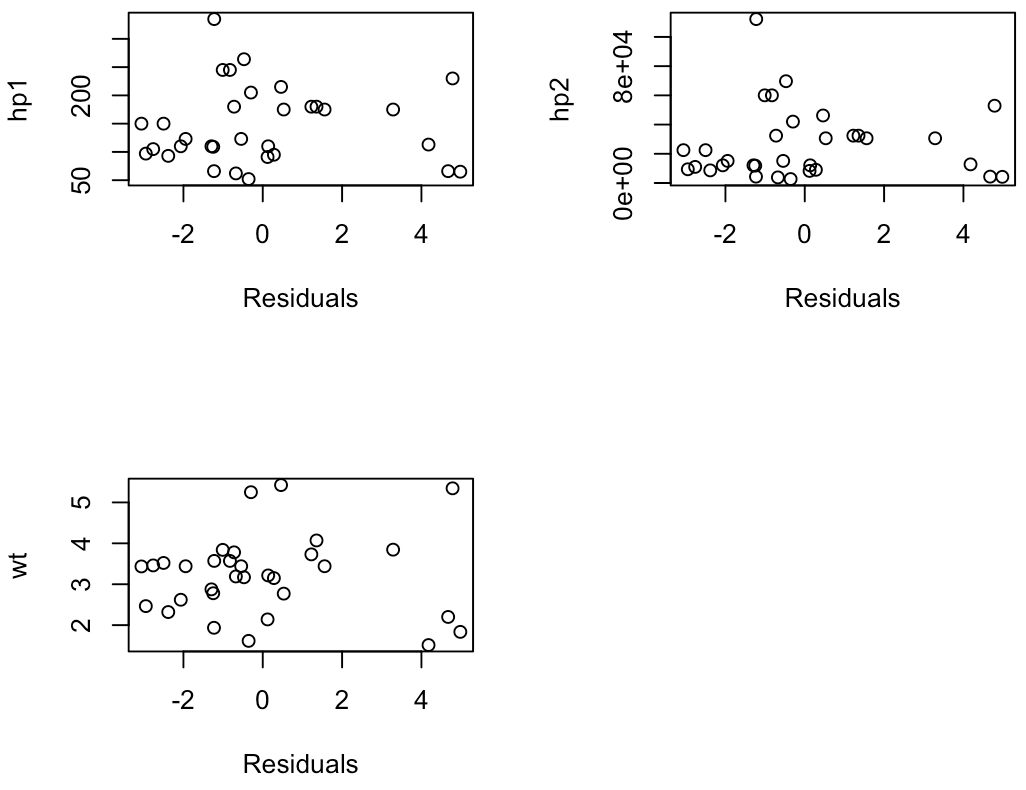
\includegraphics[width=3.5in]{images/mtcarsresidpred.png}
    \end{center}
\end{frame}
